\documentclass{standalone}
\usepackage{circuitikz}
\usepackage{schemabloc}

\begin{document}
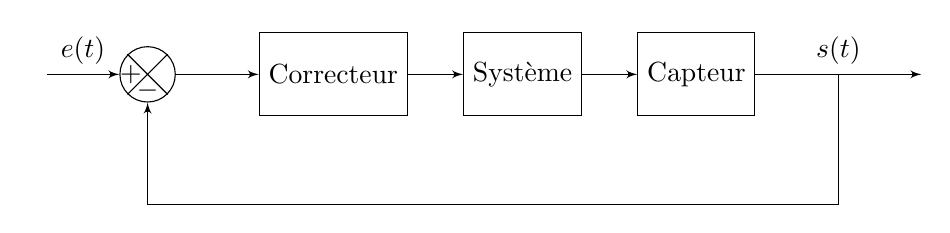
\begin{tikzpicture}
\sbEntree{E}
\sbComp{comp}{E}
\sbRelier[$e(t)$]{E}{comp}
\sbBloc[3]{B1}{Correcteur}{comp}
\sbRelier{comp}{B1}
\sbBloc{B2}{Système}{B1}
\sbRelier{B1}{B2}
\sbBloc{B3}{Capteur}{B2}
\sbRelier{B2}{B3}
\sbSortie[6]{S}{B3}
\sbRelier[$s(t)$]{B3}{S}
\sbRenvoi{B3-S}{comp}{}
\end{tikzpicture}
\end{document}